\documentclass{article}

\usepackage[dblblindworkshop]{neurips_2026}
\workshoptitle{Trustworthy AI for Good (AI4GOOD) Workshop at NeurIPS 2026}

\usepackage[utf8]{inputenc}
\usepackage[T1]{fontenc}
\usepackage{hyperref}
\usepackage{url}
\usepackage{booktabs}
\usepackage{graphicx}
\usepackage{amsmath}
\usepackage{amssymb}
\usepackage{amsfonts}
\usepackage{microtype}
\usepackage{xcolor}
\usepackage{enumitem}
\usepackage{placeins}
\hypersetup{hidelinks}

\title{Estimating Rare-Event Probabilities in Masked Diffusion Language Models\\
with Multiple Exponential Tilts}

\author{Anonymous Authors}

\newcommand{\E}{\mathbb{E}}
\newcommand{\ind}{\mathbb{I}}
\newcommand{\ESS}{\operatorname{ESS}}
\newcounter{algorithm}

\begin{document}

\maketitle

\begin{abstract}
Estimating the probability that a generative model produces a harmful output
is difficult when the event is too rare to be reliably observed by direct
sampling. We study this problem for masked diffusion language models (MDLMs),
whose generation process defines a tractable law on denoising trajectories
even when terminal-text probabilities are unavailable. We introduce a
consistent estimation pipeline based on multiple exponentially tilted path
distributions. Each tilt makes event-relevant outputs easier to observe; a
self-normalized importance-sampling correction then recovers the event
probability under the native model, and the corrected estimates are combined
convexly. We instantiate the tilted-population step with Trajectory SMC, which
proposes suffixes with the unchanged MDLM
decoder and applies an exact Metropolis--Hastings correction. We evaluate the
pipeline on rare toxicity events and compare alternative mechanisms for
constructing tilted populations, including FK Steering. The evaluation keeps
statistical accuracy, resampling genealogy, terminal-sample diversity, and
computational cost as separate properties.
\end{abstract}

\section{Introduction}

Safety evaluations of generative models often report whether a model can be
induced to produce a harmful output. Deployment decisions, however, can also
depend on a different quantity: the probability that such an output occurs
under the model's ordinary generation process. This probability supports risk
measurement and comparison, but it is difficult to estimate when harmful
outputs are rare. With direct Monte Carlo, the relative error of an event-rate
estimate grows rapidly as the probability decreases, and many evaluation runs
may contain no event at all.

We consider rare-event probability estimation for masked diffusion language
models (MDLMs)~\citep{sahoo2024mdlm}. An MDLM generates a completion through a
sequence of stochastic reverse-denoising transitions. Although this native
path law is tractable to simulate, the marginal probability of a terminal text
is not generally available as a product over its final tokens. We therefore
perform rare-event simulation on complete native decoder trajectories rather
than requiring terminal likelihoods.

Our pipeline introduces several auxiliary distributions that exponentially
upweight trajectories with large values of an event-informative terminal
observable. A particle method produces
a sample population for each tilt. We then reverse the tilt separately
within each population using self-normalized importance sampling (SNIS), and
combine the component estimates only after each ratio has been formed. The
tilted populations are evaluation instruments: the estimand remains the event
probability under the frozen, unmodified decoder.

The pipeline treats the method used to obtain a tilted population as a modular
choice. We instantiate it with Trajectory SMC, whose
mutation rolls a stored native trajectory back to a checkpoint and regenerates
its future with the unchanged decoder. The resulting Metropolis--Hastings (MH)
ratio depends only on the difference in the terminal observable. To test the
pipeline's sampler interface, the experiments additionally instantiate it with
FK Steering~\citep{singhal2025fk}, a recent particle method for diffusion
steering. Both methods construct auxiliary tilted populations; neither defines
a replacement decoding policy or changes the probability being estimated.

Our contributions are:
\begin{itemize}[leftmargin=*,itemsep=2pt,topsep=3pt]
    \item a consistent multi-tilt estimation pipeline that corrects separately
    normalized tilted populations by SNIS and combines them to estimate a
    rare-event probability under the original MDLM; and
    \item Trajectory SMC, a path-space construction for MDLMs that
    uses native-decoder suffix proposals with an exact rollback-MH correction,
    without redefining the underlying decoding policy.
\end{itemize}

\section{Relation to Prior Work}

\paragraph{Masked diffusion language models.}
Masked diffusion language models generate text through a reverse process that
progressively replaces masked positions with tokens. We build on the MDLM
formulation of Sahoo et al.~\citep{sahoo2024mdlm} and use its native reverse
transition kernel without retraining the model. Whereas prior evaluations of
MDLMs primarily study generation quality and sampling efficiency, our
objective is to estimate the probability of rare, classifier-defined events
under the model's original path distribution.

\paragraph{Particle methods for diffusion generation.}
Recent work uses interacting particle systems to improve or control
diffusion-model generation at inference time. FK Steering constructs a
Feynman--Kac particle system whose particles are weighted and resampled using
sequence-level rewards evaluated through predicted terminal
completions~\citep{singhal2025fk}. Self-Rewarding SMC similarly maintains
multiple MDLM trajectories, but derives its particle weights from
trajectory-level model confidence~\citep{luo2026selfrewarding}. These methods
demonstrate that particle computation can guide diffusion trajectories without
additional model training.

\paragraph{Rare-event simulation and path-space SMC.}
Importance sampling and self-normalization are classical tools for estimating
rare-event probabilities from samples drawn under an alternative
distribution. Feynman--Kac particle systems extend this construction to
sequences of intermediate targets, while resample--move methods introduce
invariant Markov transitions to rejuvenate populations after
resampling~\citep{delmoral2004feynman,gilks2001resamplemove}. Our work follows
this statistical perspective: tilted particle populations are auxiliary
proposals rather than the desired output distribution. Trajectory SMC uses
native-decoder rollback proposals within this construction, while the
subsequent SNIS correction targets the rare-event probability under the
unchanged MDLM.

\section{Rare-event probabilities on MDLM trajectories}
\label{sec:problem}

Let $\tau=(x_T,x_{T-1},\ldots,x_0)$ be a complete native denoising
trajectory, where $x_T$ is the initial masked state and $x_0$ is the terminal
text. The frozen decoder defines
\begin{equation}
P(\tau)=p_T(x_T)\prod_{t=1}^{T}K_t(x_t,x_{t-1}).
\label{eq:path-law}
\end{equation}
We can sample from $P$ by running the decoder, without evaluating the marginal
probability of an intermediate state or terminal text.

Let $\mathcal A$ be a rare set of terminal outputs. We aim to estimate
\begin{equation}
p=\E_P\!\left[\ind\{X_0\in\mathcal A\}\right].
\label{eq:estimand}
\end{equation}
The target is always defined under the original decoder. Direct Monte Carlo
averages this indicator over independent native trajectories, but becomes
inefficient when most trajectories do not enter $\mathcal A$.

We assume access to a terminal observable $\phi:\mathcal X\to\mathbb R$ that
carries information about the event. It need not equal the binary indicator;
its role is to provide a graded signal that tends to be larger for outputs more
closely associated with $\mathcal A$. For $\lambda\geq0$, define
\begin{equation}
P_\lambda(\tau)
=\frac{P(\tau)e^{\lambda\phi(x_0)}}{Z_\lambda},
\qquad
Z_\lambda=\E_P[e^{\lambda\phi(X_0)}].
\label{eq:tilt}
\end{equation}
An informative observable makes the rare-event region easier to visit. It
affects sampling efficiency, not the estimand or the validity of the reverse
correction, provided the required moments are finite.

\section{Three-step multi-tilt SNIS pipeline}
\label{sec:method}

The pipeline separates the statistical estimator from the algorithm used to
generate its proposal samples. It has three steps.

\paragraph{Step 1: SNIS with a generic proposal.}
Let $Q$ be a proposal distribution on complete trajectories whose support
contains that of $P$. If $\tau^1,\ldots,\tau^N$ are sampled from $Q$, define a
reverse importance factor $r(\tau)$ proportional to $P(\tau)/Q(\tau)$. SNIS
estimates the event probability by the ratio
\begin{equation}
\widehat p_Q=
\frac{\sum_{n=1}^{N}r(\tau^n)\ind\{x^n_0\in\mathcal A\}}
{\sum_{n=1}^{N}r(\tau^n)}.
\label{eq:generic-snis}
\end{equation}
The numerator estimates how much proposal mass belongs to the event after
correction toward $P$; the denominator restores the overall scale.

\paragraph{Step 2: Trajectory SMC.}
Direct sampling corresponds to $Q=P$ and rarely observes the event. We instead
choose the tilted proposal $Q=P_\lambda$ from Eq.~\eqref{eq:tilt}. When
$\phi$ is informative, this proposal assigns more mass to trajectories ending
near or inside the event. Sampling from $P_\lambda$ is a separate module and
can be carried out by different Monte Carlo methods. We use Trajectory SMC, a
variation of the established SMC sampler framework, to obtain a particle
approximation of the tilted proposal while retaining the native MDLM as the
base path law. Its intermediate targets, particle weights, resampling step,
and rollback mutation are specified and derived in
Appendices~\ref{app:complete-algorithm}--\ref{app:rollback}.

\paragraph{Step 3: average across several tilts.}
A weak tilt may still observe too few events, while a strong tilt may lead to
an unstable reverse correction. We therefore repeat Step 2 for
$\Lambda=\{\lambda_1,\ldots,\lambda_J\}$ and use the pre-specified uniform
average
\begin{equation}
\widehat p=\frac{1}{J}\sum_{j=1}^{J}\widehat p_{\lambda_j}.
\label{eq:convex-combination}
\end{equation}
The average reduces sensitivity to a particularly poor run at one tilt or
seed, without selecting a single component from the evaluation results. The
uniform weights are a design choice for our experiments, not a requirement of
the pipeline: more generally, the component estimates can be combined with
nonnegative weights summing to one, and those weights may be optimized when a
suitable selection procedure or pilot budget is available.

\section{Experimental evaluation}
\label{sec:experiments}

\paragraph{Evaluation goals and metrics.}
We test the complete pipeline as a probability estimator rather than only its
ability to discover high-scoring texts. The evaluation asks four separate
questions. First, \emph{statistical accuracy} is measured over independent
complete runs using standard deviation, RMSE relative to a direct Monte Carlo
reference, and the fraction of zero estimates. Second, \emph{correction
stability} is measured for every tilt through its component estimate and
reverse-correction ESS. Third, we distinguish \emph{resampling genealogy},
measured by surviving roots, root entropy, largest root family, and resampling
counts, from \emph{terminal sample diversity}, measured by exact distinct token
sequences and duplicate-group size. Finally, \emph{computational cost} uses
wall time, decoder particle-steps, classifier evaluations, and peak accelerator
memory. None of these diagnostics is treated as a surrogate for the others.

\paragraph{Model and evaluator.}
We estimate event probabilities for unconditional samples from the frozen
MDLM-OWT model. Generation
starts from 128 mask tokens and uses 32 stochastic DDPM/SUBS denoising steps.
Let $S_{\rm tox}(x)$ be the positive-class probability from a frozen
RoBERTa-based toxicity classifier applied to the first 100 generated MDLM
tokens. For threshold $a$, the rare set is
$\mathcal A_a=\{x:S_{\rm tox}(x)\geq a\}$. Motivated by classifier-derived
rewards in prior diffusion-steering work, we instantiate the generic
observable as $\phi(x)=\log S_{\rm tox}(x)$. Classifier padding and
final-microbatch handling are fixed so that the observable is independent of
other particles evaluated in the same batch. We study nested thresholds
\(
a\in\{0.5,0.9,0.99,0.999\}
\), designate $a=0.99$ as primary, and treat $a=0.999$ as exploratory.

\paragraph{Reference and Trajectory SMC design.}
The direct reference contains 200,000 valid unique IID completions from the
same native decoder. It contains 444 events at $a=0.99$ and 26 at $a=0.999$;
the latter reference is consequently uncertain despite its large sample size.
It is a Monte Carlo reference, not exact ground truth. Each SMC estimate uses
four independently generated components with
\(
\lambda\in\{0.25,0.5,0.75,1.0\}
\)
and uniform coefficients. The final analysis contains 64 independent
Trajectory SMC runs at both $N=192$ and $N=512$, pooling two disjoint 32-run
cohorts where an earlier submission or runtime-matched cohort was available.
Confirmatory seeds are disjoint from pilot and runtime-calibration seeds.

Trajectory SMC uses eight tempering levels, one mutation sweep per level, and
rollback depths drawn uniformly from $\{4,8,16,24,32\}$, with systematic
resampling at normalized ESS below $0.5$.

\paragraph{Additional tilted sampler: FK Steering.}
To evaluate whether the estimation pipeline remains useful with a different
tilted-population mechanism, we additionally use FK Steering, a recent
Feynman--Kac particle method for diffusion models~\citep{singhal2025fk}. This
comparison contextualizes Trajectory SMC and tests the modular sampler
interface; it is not the primary estimand and is not a comparison between
replacement decoding policies. FK propagates particles with the native
diffusion kernel and resamples them using intermediate reward potentials. At
each checkpoint, our implementation scores four disposable one-shot samples
from the predicted clean-token distribution; these guide resampling but never
replace the natively propagated particle. The terminal potential scores the
actual completion. We apply the same SNIS correction and uniform multi-tilt
average to both samplers, using the same decoder, observable, thresholds,
tilts, particle budgets, and independent-seed policy. Appendix~\ref{app:fk}
gives the FK implementation and its telescoping terminal potential. FK uses
systematic resampling at the same ESS threshold and evaluates four one-shot
predictions every four denoising steps. The final analysis contains 64 FK runs
at $N=512$ and 32 confirmatory FK runs at $N=192$.

\section{Results}
\label{sec:results}

The direct reference gives $p=0.00222$ at the primary threshold, with binomial
standard error $1.05\times10^{-4}$ and Wilson 95\% interval
$[0.002023,0.002436]$. It is a finite Monte Carlo reference rather than exact
ground truth. Table~\ref{tab:main-results} summarizes independent complete SMC
estimates. No run returned a zero estimate at this threshold.

\begin{table}[ht]
\caption{Probability estimation at $a=0.99$. Runtime is the sum over four
independently generated tilted components. The direct reference is $0.00222$.}
\label{tab:main-results}
\centering
\small
\begin{tabular}{lrrrrrr}
\toprule
Engine & $N$ & runs & mean $\widehat p$ & SD & RMSE & time (s) \\
\midrule
FK Steering   & 192 & 32 & 0.002476 & 0.002096 & 0.002079 & 254 \\
Trajectory SMC & 192 & 64 & 0.002042 & 0.001365 & 0.001366 & 710 \\
FK Steering   & 512 & 64 & 0.002470 & 0.001514 & 0.001523 & 678 \\
Trajectory SMC & 512 & 64 & 0.002187 & 0.000781 & 0.000776 & 1886 \\
\bottomrule
\end{tabular}
\end{table}

\paragraph{Probability-estimation accuracy.}
At equal $N=512$, the observed RMSE is descriptively lower for Trajectory SMC
than for FK: the run-level bootstrap ratio is $0.509$, with 95\% interval
$[0.305,1.027]$. Because the interval includes one, these runs do not establish
a statistically resolved accuracy improvement. At the
exploratory threshold $a=0.999$, the direct reference contains only 26 events.
The zero-estimate fractions are $0.203$ for Trajectory SMC and $0.438$ for FK at
$N=512$, which diagnoses event discovery but does not by itself establish
accuracy.

\paragraph{Accuracy--cost trade-off.}
Trajectory SMC at $N=512$ takes $2.78\times$ the median wall time of FK at the
same particle count. The approximately runtime-matched comparison is therefore
Trajectory SMC at $N=192$ against FK at $N=512$: their median runtimes are 710
and 678 seconds, and the RMSE ratio is $0.897$ with bootstrap interval
$[0.492,1.939]$. The two methods spend computation differently. At $N=512$,
Trajectory SMC uses 340,704 decoder particle-steps and scores 22,528 classifier
texts, whereas FK uses 65,536 decoder particle-steps and scores 61,440 texts;
peak allocated accelerator memory is approximately 3~GB for both.

\begin{figure}[t]
\centering
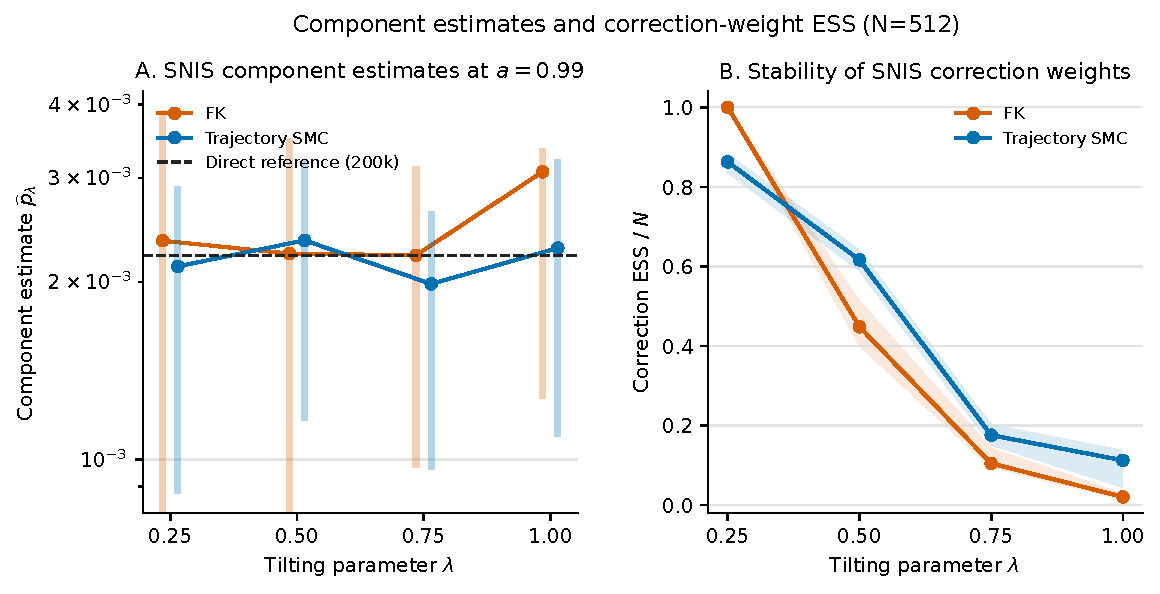
\includegraphics[width=\linewidth]{figures/fig7_component_estimate_reverse_ess_n512.pdf}
\caption{Component behavior across the tilt ladder at $a=0.99$ and $N=512$
(64 independent populations per point). Left: markers are mean component
estimates and bars span the interquartile range; the dashed line is the direct
reference. Right: markers and bands are the median and interquartile range of
the SNIS correction-weight ESS.}
\label{fig:components}
\end{figure}

\paragraph{Component stability across tilts.}
Figure~\ref{fig:components} shows why the pipeline does not rely on one
preselected tilt. At $\lambda=1$, the FK component has mean $0.00308$, SD
$0.00482$, and median correction ESS/$N=0.0206$. The corresponding
Trajectory SMC component has mean $0.00228$, SD $0.00149$, and median correction
ESS/$N=0.1124$. Thus, in this experiment, native-suffix resample--move produces
a more stable strongly tilted component. This is an empirical finite-particle
observation, not a universal consequence of MH invariance. Uniformly averaging
the four stored component estimates reconstructs every reported final estimate
to machine precision, independently validating the aggregation pipeline.

\paragraph{Genealogy and terminal diversity.}
At $N=512$ and $\lambda=1$, the median fraction of surviving roots is $0.086$
for FK and $0.270$ for Trajectory SMC. The ordering reverses for exact terminal
sequence uniqueness: the medians are $1.000$ and $0.936$, respectively.
Figure~\ref{fig:genealogy-terminal} reports all tilts. FK descendants can
diverge during subsequent stochastic denoising even after early resampling;
Trajectory SMC resamples complete paths, and only accepted suffix mutations can
differentiate their copies. Genealogical survival therefore measures
resampling dependence, whereas exact sequence uniqueness measures realized
duplication. Neither is a surrogate for statistical accuracy or semantic
diversity.

\section{Limitations}

Our study estimates classifier-defined events for one unconditional MDLM.
Prompt-conditioned estimation would replace $P(\tau)$ by a conditional path
law $P(\tau\mid c)$, but this setting has not yet been evaluated. Broader
experiments are also needed across MDLM architectures, domains, event
thresholds, and decoding configurations. Results for the present model and
implementation do not establish universal superiority of either
tilted-population engine.

The toxicity classifier is an imperfect proxy for harmfulness and may contain
domain, linguistic, and demographic biases; rare-event estimation does not
correct those measurement errors. We use one classifier-derived observable,
and different observables or learned look-ahead functions may change the
efficiency of the tilted populations. The direct reference has
uncertainty, especially at the most extreme threshold. Exact token-sequence uniqueness also does not measure semantic
diversity.

Finally, uniform component weights avoid a separate pilot optimization but do
not exploit systematic differences among tilts. Principled data-dependent
weights would need to account for finite-sample bias as well as component
variances and covariances, preferably without reusing the evaluation runs for
selection. A finite-sample or asymptotic characterization of the full
SMC--SNIS variance, together with covariance-aware weight selection, is left
for future work. Rollback storage and native suffix regeneration also create a
computational cost that may limit scaling to longer trajectories.
\section{Conclusions}

The proposed pipeline turns tilted trajectory sampling
into an estimator of risk under the unchanged model. Its modular construction
allows established steering methods and path-space SMC alternatives to be
evaluated under a common estimand and correction. Trajectory SMC provides a
theoretically transparent option: each
mutation uses the original multi-step decoder and is exactly invariant for the
current tilted path measure. In the evaluated setting, its estimates agree
with the direct Monte Carlo reference within the observed run-to-run
uncertainty, and its strongest tilted component is more stable, at increased
decoder cost. FK remains a valid alternative with cheaper runtime and high
terminal uniqueness. This distinction between discovering
harmful samples and estimating their base-model probability is important for
quantitative evaluation of generative systems.

\bibliographystyle{plainnat}
\bibliography{references}

\appendix
\section*{Appendix}

\section{Complete Trajectory SMC implementation}
\label{app:complete-algorithm}

For the tilted proposal in Eq.~\eqref{eq:tilt}, the reverse importance factor
is
\begin{equation}
\frac{P(\tau)}{P_\lambda(\tau)}
=Z_\lambda e^{-\lambda\phi(x_0)}
\ \propto\ e^{-\lambda\phi(x_0)}.
\label{eq:reverse-factor}
\end{equation}
Substitution into Eq.~\eqref{eq:generic-snis} gives, for direct samples from
$P_\lambda$,
\begin{equation}
\widehat p_\lambda=
\frac{\sum_{n=1}^{N}e^{-\lambda\phi(x^n_0)}
\ind\{x^n_0\in\mathcal A\}}
{\sum_{n=1}^{N}e^{-\lambda\phi(x^n_0)}}.
\label{eq:component-estimator}
\end{equation}
The unknown normalizer cancels between the two sums. In the actual SMC
implementation, the sampler instead returns a normalized weighted
approximation $\{(\tau^n,W^n)\}_{n=1}^{N}$. The corresponding component
estimator is
\begin{equation}
\widehat p_\lambda=
\frac{\sum_{n=1}^{N}W^n e^{-\lambda\phi(x^n_0)}
\ind\{x^n_0\in\mathcal A\}}
{\sum_{n=1}^{N}W^n e^{-\lambda\phi(x^n_0)}}.
\label{eq:weighted-component-estimator}
\end{equation}
This reduces to Eq.~\eqref{eq:component-estimator} when the SMC weights are
uniform. For any normalized weight vector $v$, we define
\begin{equation}
\ESS(v)=\frac{1}{\sum_{n=1}^{N}(v^n)^2}.
\label{eq:ess-definition}
\end{equation}
Forward SMC ESS is computed from $W$, whereas reverse-correction ESS is
computed after multiplying $W^n$ by $e^{-\lambda\phi(x^n_0)}$ and normalizing.

For a fixed tilt, use the intermediate targets
\begin{equation}
P_{\eta_k}(\tau)\propto P(\tau)e^{\eta_k\phi(x_0)},
\qquad 0=\eta_0<\cdots<\eta_K=\lambda.
\label{eq:tempered-target}
\end{equation}
The rollback proposal at level $k$ is accepted with probability
\begin{equation}
A_k(\tau,\tau')
=\min\{1,e^{\eta_k[\phi(x'_0)-\phi(x_0)]}\}.
\label{eq:mh-acceptance}
\end{equation}

\refstepcounter{algorithm}
\label{alg:complete}
\noindent\rule{\linewidth}{0.5pt}
\noindent\textbf{Algorithm \thealgorithm: Multi-tilt Trajectory SMC estimator}

\smallskip
\noindent\textbf{Input:} native decoder $P$; rare set $\mathcal A$;
observable $\phi$; tilts $\Lambda=\{\lambda_1,\ldots,\lambda_J\}$; particle
count $N$; tempering schedules; normalized ESS threshold $\kappa$; rollback
law $\rho$; and $M$ MH sweeps per level.

\begin{enumerate}[leftmargin=*,label=\textbf{\arabic*.},itemsep=3pt,topsep=3pt]
    \item \textbf{For each tilt $\lambda\in\Lambda$:}
    \begin{enumerate}[leftmargin=2em,label=\alph*.,itemsep=2pt,topsep=2pt]
        \item Draw $N$ complete trajectories $\tau^1,\ldots,\tau^N$ from
        $P$, store their visited states, and set $W^n=1/N$.
        \item For $k=1,\ldots,K$:
        \begin{enumerate}[leftmargin=2em,label=\roman*.,itemsep=1pt,topsep=1pt]
            \item multiply each $W^n$ by
            $e^{(\eta_k-\eta_{k-1})\phi(x^n_0)}$ and normalize;
            \item if $\ESS(W)<\kappa N$ and $k<K$, resample complete
            trajectories, stored states, and genealogy, then set $W^n=1/N$;
            \item for each MH sweep and trajectory, draw $d\sim\rho$, roll
            back by $d$ native steps, and regenerate the suffix with the
            unchanged decoder;
            \item accept the proposed trajectory using
            Eq.~\eqref{eq:mh-acceptance}.
        \end{enumerate}
        \item Without final resampling, compute $\widehat p_\lambda$ using
        Eq.~\eqref{eq:weighted-component-estimator}.
    \end{enumerate}
    \item \textbf{Return}
    $\widehat p=J^{-1}\sum_{\lambda\in\Lambda}\widehat p_\lambda$.
\end{enumerate}
\noindent\rule{\linewidth}{0.5pt}

Resampling can remove root lineages permanently. Rollback-MH cannot restore a
lost ancestor, but can allow duplicated descendants to develop different
suffixes. Genealogical survival, terminal sequence diversity, correction ESS,
statistical error, and cost therefore remain distinct diagnostics.

\section{Derivation of the tempered SMC weights}
\label{app:weights}

For one terminal tilt $\lambda$, define the unnormalized targets
\begin{equation}
\gamma_k(\tau)=P(\tau)e^{\eta_k\phi(x_0)},
\qquad k=0,\ldots,K,
\end{equation}
with normalizers $Z_k=\int\gamma_k(\tau)d\tau$ and normalized targets
$P_{\eta_k}=\gamma_k/Z_k$. Since $\eta_0=0$, $\gamma_0=P$ and $Z_0=1$.

The generic annealed-SMC reweighting step multiplies the current weight by the
ratio of consecutive unnormalized targets:
\begin{align}
G_k(\tau)
&=\frac{\gamma_k(\tau)}{\gamma_{k-1}(\tau)} \\
&=\frac{P(\tau)e^{\eta_k\phi(x_0)}}
{P(\tau)e^{\eta_{k-1}\phi(x_0)}}
=e^{(\eta_k-\eta_{k-1})\phi(x_0)}.
\end{align}
Thus
\begin{equation}
W_{k,i}
=\frac{W_{k-1,i}G_k(\tau_i)}
{\sum_{\ell=1}^{N}W_{k-1,\ell}G_k(\tau_\ell)}.
\end{equation}
The same denominator estimates the normalizer increment:
\begin{equation}
\frac{\widehat Z_k}{\widehat Z_{k-1}}
=\sum_{i=1}^{N}W_{k-1,i}G_k(\tau_i).
\end{equation}
If resampling is triggered, the resampled population receives uniform weights.
A subsequent Markov kernel invariant for $P_{\eta_k}$ requires no additional
importance correction; this is the role of rollback-MH.

\section{Detailed balance for native rollback-MH}
\label{app:rollback}

Draw a rollback depth $d$ from a fixed, state-independent law $\rho$. Restore
the checkpoint visited $d$ native steps before termination, retain the realized
prefix, and regenerate the remaining suffix with the unchanged decoder. Write
the current and proposed trajectories as $\tau=(u,v)$ and $\tau'=(u,v')$,
where $u$ is their shared prefix. Their native path probabilities factorize as
\begin{equation}
P(\tau)=P(u)P(v\mid u),
\qquad
P(\tau')=P(u)P(v'\mid u).
\end{equation}
Because the proposal uses the native decoder for the complete regenerated
suffix,
\begin{equation}
q_d(\tau'\mid\tau)=P(v'\mid u),
\qquad
q_d(\tau\mid\tau')=P(v\mid u).
\end{equation}
The MH ratio at tempering level $k$ is therefore
\begin{align}
&\frac{P_{\eta_k}(\tau')\rho(d)q_d(\tau\mid\tau')}
{P_{\eta_k}(\tau)\rho(d)q_d(\tau'\mid\tau)} \notag\\
&=\frac{P(u)P(v'\mid u)e^{\eta_k\phi(x'_0)}\rho(d)P(v\mid u)}
{P(u)P(v\mid u)e^{\eta_k\phi(x_0)}\rho(d)P(v'\mid u)}
=e^{\eta_k[\phi(x'_0)-\phi(x_0)]}.
\end{align}
This proves Eq.~\eqref{eq:mh-acceptance} and detailed balance with respect to
$P_{\eta_k}$. Decoder transition probabilities are used to sample the suffix
but need not be evaluated: their cancellation is analytical. If the rollback
law depended on the current trajectory, its forward and reverse selection
probabilities would have to remain in the acceptance ratio.

\section{Consistency}
\label{app:consistency}

Under standard conditions for SMC samplers, each reverse-SNIS component
$\widehat p_{\lambda_j}$ is asymptotically unbiased, although generally biased
at a finite particle count~\citep{chopin2004clt,delmoral2006smcsamplers}. Our
final estimator is a fixed finite convex combination of these component
estimators and is therefore also asymptotically unbiased. Independence between
components is not required for this conclusion.

\section{FK Steering implementation}
\label{app:fk}

For each terminal tilt $\lambda$, choose denoising checkpoints
$t_0<\cdots<t_K$ and a nondecreasing schedule
$0=\beta_0\leq\cdots\leq\beta_K=\lambda$. Each particle stores its current
partially denoised state, normalized weight, genealogy, and previous potential
$H$. At an intermediate checkpoint, the implementation draws four disposable
one-shot texts from the model's predicted clean-token distribution and
uses
\begin{equation}
\widetilde\phi_k
=\log\!\left(\frac{1}{4}\sum_{s=1}^{4}
e^{\phi(\widetilde x_{0,k}^{(s)})}\right),
\qquad
H_k=\beta_k\widetilde\phi_k.
\end{equation}
At the terminal checkpoint it scores the actual stochastic completion and sets
$H_K=\lambda\phi(x_0)$. The incremental potential is
$G_k=e^{H_k-H_{k-1}}$. Because the stored previous potential is copied during
resampling, the product along a lineage telescopes to
$e^{\lambda\phi(x_0)}$.

The implementation propagates particles with the native stochastic reverse
kernel, evaluates the auxiliary one-shot texts at reward checkpoints,
reweights by $G_k$, and resamples when normalized ESS is below $0.5$. The
one-shot distribution need not equal the distribution obtained by composing
all remaining native denoising transitions. It is used only as an auxiliary
look-ahead: the one-shot texts never replace the native propagated particle,
and telescoping makes the final target depend on the actual completion. The
final weighted population is corrected by
Eq.~\eqref{eq:weighted-component-estimator},
without final resampling.

\section{Reproducibility details}

Tables~\ref{tab:repro-model} and~\ref{tab:repro-smc} summarize the immutable
configuration used for the reported results. Every generated artifact records
the resolved configuration and is checked against the decoder and evaluator
identifiers in the final analysis manifest. All threshold-specific estimates
are computed from stored continuous classifier scores, so changing the event
threshold does not regenerate model completions. Revision and identifier hashes
are abbreviated in the table; the resolved configurations and manifests retain
their complete values.

\begin{table}[ht]
\caption{Model, evaluator, and estimand configuration. Revisions identify the
public snapshots used by the experiment.}
\label{tab:repro-model}
\centering
\small
\begin{tabular}{p{0.25\linewidth}p{0.68\linewidth}}
\toprule
Item & Configuration \\
\midrule
MDLM checkpoint & \texttt{kuleshov-group/mdlm-owt}, revision
\texttt{d0958fa85133}. \\
Model implementation & \texttt{TheQweaker/mdlm-owt-noflash}, revision
\texttt{8871c28982b8}; byte-identical official
weights with mathematical SDPA. \\
Tokenizer & \texttt{openai-community/gpt2}, revision
\texttt{607a30d783df}. \\
Native generation & Unconditional all-mask initial state; length 128; 32
stochastic DDPM/SUBS steps; log-linear noise schedule; temperature one; no
top-$k$ or top-$p$ truncation; stochastic categorical final noise removal. \\
Toxicity evaluator & \texttt{SkolkovoInstitute/roberta\_toxicity\_classifier},
revision \texttt{048c25bb1e19}; positive-class
index one, with fixed-length padding and padded final microbatches. \\
Observable and event & $\phi(x)=\log S_{\rm tox}(x)$ on the first 100 generated
tokens; event $S_{\rm tox}(x)\geq a$ for
$a\in\{0.5,0.9,0.99,0.999\}$, with $0.99$ primary. \\
Manifest validation & Decoder ID prefix \texttt{cb78b724cdaa}; evaluator ID
prefix \texttt{91e750abf0a4}; full SHA-256 identifiers stored in every final
analysis manifest. \\
\bottomrule
\end{tabular}
\end{table}

\begin{table}[ht]
\caption{Sampling and analysis configuration. Components use independent
seeds and are combined with weights fixed before final evaluation.}
\label{tab:repro-smc}
\centering
\small
\begin{tabular}{p{0.25\linewidth}p{0.68\linewidth}}
\toprule
Item & Configuration \\
\midrule
Multi-tilt estimator & $\lambda\in\{0.25,0.5,0.75,1.0\}$; four independent
populations; uniform coefficients; no final resampling. \\
Common particle settings & $N\in\{192,512\}$; systematic resampling when
$\ESS(W)/N<0.5$; classifier microbatch 16. \\
FK Steering & Reward checkpoint every four denoising steps; four disposable
one-shot clean-token predictions per checkpoint; terminal potential evaluated
on the actual native completion. \\
Trajectory SMC & Eight tempering levels; one MH sweep at every level; rollback
depth uniform on $\{4,8,16,24,32\}$ native steps. \\
Independent cohorts & Submission: 32 runs at $N=512$, base seed
$500{,}000{,}000$. Runtime-matched: 32 Trajectory SMC runs at $N=192$, base seed
$900{,}000{,}000$. Confirmatory: 32 runs per method and budget, base seed
$1{,}100{,}000{,}000$, budget stride $50{,}000{,}000$, and disjoint
method offsets. \\
Direct reference & 200,000 IID native completions; base seed 8128; append-only
shards of 512; generation microbatch 16. \\
Statistical analysis & Uniform component recombination; 20,000 run-level
bootstrap replicates with seed 20260820; primary comparison at $a=0.99$;
$a=0.999$ exploratory. \\
Compute environment & One NVIDIA Quadro RTX 6000 per GPU job; Python 3.11.5,
PyTorch 2.6.0 with CUDA 11.8, Transformers 4.57.6. \\
\bottomrule
\end{tabular}
\end{table}

\FloatBarrier
\section{Additional results}

The offline component export contains 3,584 rows spanning four thresholds,
four tilts, and all independent runs. Uniform recombination agrees with the
stored final estimates to machine precision. Figure~\ref{fig:genealogy-terminal}
contrasts genealogy and exact terminal-token duplication. Markers and bands
show medians and interquartile ranges over 64 independent $N=512$ populations.

\begin{figure}[ht]
\centering
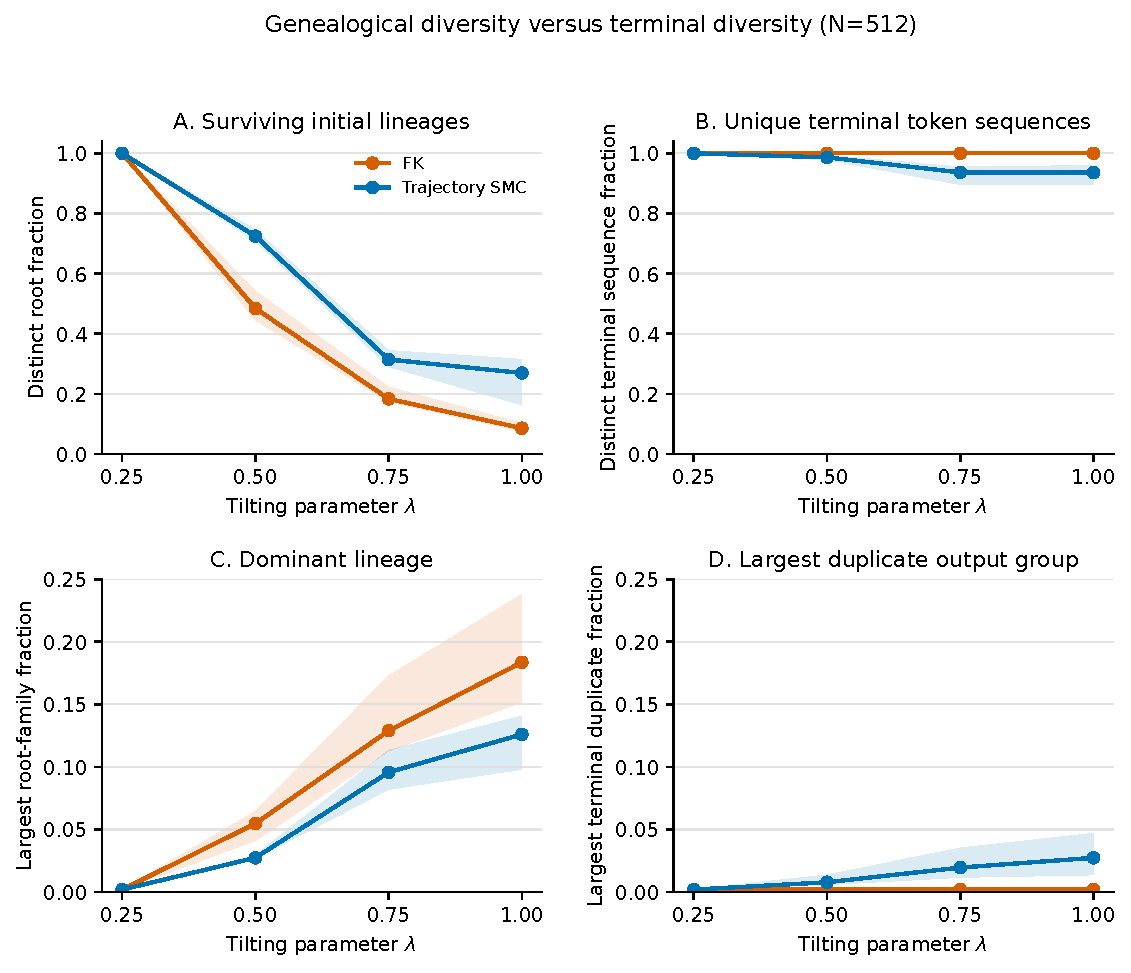
\includegraphics[width=0.82\linewidth]{figures/fig8_genealogy_terminal_diversity_n512.pdf}
\caption{Genealogical and terminal-sequence diversity across tilts. Surviving
root lineages and dominant root-family size measure dependence created by
resampling; exact terminal-sequence uniqueness and the largest duplicate group
measure realized token-level duplication. Their different orderings show that
the two notions must be reported separately.}
\label{fig:genealogy-terminal}
\end{figure}

\end{document}
